\chapter{Control del ciclo celular y muerte celular programada}\label{ch:b3:cell-cycle-apoptosis}

Unos cien mil millones de células de su cuerpo morirán hoy, a propósito,
y otros cien mil millones nacerán para reemplazarlas; el revestimiento
del intestino se renueva cada cinco días y los glóbulos rojos cada cuatro
meses. Un renacuajo pierde la cola sin sangrar; la membrana entre los
dedos de un embrión humano desaparece en la octava semana; la mitad de
las neuronas que llega a fabricar un cerebro muere antes del nacimiento.
Cada una de estas muertes la ejecuta la propia célula, siguiendo un
programa, y cada uno de los nacimientos lo autoriza un sistema de control
que decide, en dos o tres puntos del ciclo, si la célula puede seguir
adelante. Los dos programas --- división y suicidio --- son el asunto de
este capítulo. Se resolvieron en levaduras, huevos de rana, erizos de mar
y un gusano con exactamente $1090$ células somáticas de las que mueren
exactamente $131$, y resultaron ser los mismos en el ser humano, donde
sus fallos son el cáncer por un lado y la degeneración por el otro.

\section{El motor del ciclo}

\begin{definition}[Ciclinas y quinasas dependientes de ciclina]\label{def:b3:cell-cycle-apoptosis:cdk}
\index{ciclina}\index{quinasa dependiente de ciclina}\index{complejo promotor de la anafase}\index{ciclo celular}
El ciclo celular --- G1, S (replicación), G2, M (mitosis) --- lo impulsa
una familia de proteína-quinasas, las \emph{quinasas dependientes de
ciclina} (CDK), cuyas subunidades catalíticas están presentes a lo largo
de todo el ciclo pero solo son activas cuando se unen a una
\emph{ciclina}, una subunidad reguladora cuya concentración sube y baja
en un orden fijo: la ciclina D con Cdk4/6 en G1 en respuesta a factores
de crecimiento, la ciclina E con Cdk2 en la transición G1/S, la ciclina A
con Cdk2 a lo largo de S y la ciclina B con Cdk1 en la entrada en
mitosis. Cada pareja ciclina--CDK fosforila las proteínas de su fase ---
orígenes de replicación, laminas, condensinas, enzimas del ensamblaje del
huso --- y cada una se apaga con la destrucción de su ciclina: unas
ubiquitina-ligasas (SCF en G1/S y el \emph{complejo promotor de la
anafase}, APC/C, en mitosis) marcan las ciclinas para el proteasoma. La
actividad de Cdk1 está además regulada por una fosforilación inhibidora
que pone la quinasa Wee1 y quita la fosfatasa Cdc25, y por pequeñas
proteínas inhibidoras (p21, p27, p16) que se unen a los complejos. El
ciclo es así una secuencia ordenada de oleadas de quinasa, cada una de
las cuales termina con la proteólisis de lo que la produjo.
\end{definition}

\begin{proof}[Evidencia]
Convergieron tres líneas. Hartwell (años setenta) aisló mutantes
\emph{cdc} de la levadura de gemación sensibles a la temperatura, cada
uno detenido en una etapa con un tamaño de yema característico, y definió
\emph{Start}, el punto de G1 a partir del cual una célula queda
comprometida con un ciclo. Nurse (años ochenta) descubrió en la levadura
de fisión que \emph{cdc2} controlaba el momento de la mitosis y que el
gen humano, introducido en la levadura, rescataba al mutante: la quinasa
era Cdk1, conservada de la levadura al hombre. Hunt (1983) encontró en
huevos de erizo de mar una proteína que se acumulaba a lo largo de cada
ciclo y se destruía de golpe en cada división, y la llamó \omterm{def:b3:cell-cycle-apoptosis:cdk}{ciclina}. El
huevo de rana había dado entretanto un ``factor promotor de la
maduración'' que empujaba a cualquier núcleo a la mitosis; era la \omterm{def:b3:cell-cycle-apoptosis:cdk}{ciclina}
B unida a Cdk1. Rao y Johnson (1970) habían mostrado, fusionando células,
que una célula en fase S empuja a un núcleo en G1 a replicar, mientras
que un núcleo en G2 espera --- el citoplasma lleva la señal, y a un
núcleo ya replicado no se le puede hacer replicar de nuevo.
\end{proof}

\begin{omfigure}
\begin{tikzpicture}[every node/.style={font=\scriptsize}, >=stealth]
  % cycle circle with phases
  \draw[very thick, omDef!50] (0,0) circle (2.2);
  \foreach \a/\b/\col/\lab/\r in {90/200/omDef!25/G1/1.55, 200/270/omProp!30/S/1.55, 270/315/omMeth!30/G2/1.55, 315/450/omThm!30/M/1.55} {
    \fill[\col] (0,0) -- (\a:2.2) arc[start angle=\a, end angle=\b, radius=2.2] -- cycle;
    \node[font=\small\bfseries] at ({(\a+\b)/2}:\r) {\lab};
  }
  \fill[white] (0,0) circle (1.0);
  \draw[very thick, omDef!50] (0,0) circle (2.2);
  % cyclin-CDK labels around
  \node[left, align=right] at (-2.4,1.2) {ciclina D--Cdk4/6\\factores de crecimiento, Rb apagada};
  \node[left, align=right] at (-2.4,-1.0) {ciclina E--Cdk2\\disparan los orígenes};
  \node[anchor=north east, align=right] at (-1.3,-2.2) {ciclina A--Cdk2\\replicación};
  \node[right, align=left] at (2.4,-1.0) {ciclina B--Cdk1\\entrada en mitosis};
  \node[right, align=left] at (2.4,1.3) {el APC/C destruye la ciclina B\\y la securina: anafase, salida};
  % checkpoints as bars
  \foreach \a in {160,270,20} \draw[very thick, omThm] (\a:1.95) -- (\a:2.45);
  \node[align=center, anchor=south east] at (-1.2,2.35) {punto de restricción:\\¿hay factores de crecimiento?};
  \node[align=left, anchor=west] at (2.55,0.35) {punto de control del huso:\\¿todos los cinetocoros unidos?};
  \node[align=center, anchor=north] at (1.5,-2.55) {punto de control G2/M:\\¿ADN intacto?};
  \draw[->, thick] (0,0) ++(60:1.25) arc[start angle=60, end angle=30, radius=1.25];
\end{tikzpicture}

{\small El ciclo como una secuencia de oleadas de ciclina--CDK, cada una
terminada por la destrucción de su \omterm{def:b3:cell-cycle-apoptosis:cdk}{ciclina}, con los tres \omterm{def:b3:cell-cycle-apoptosis:checkpoints}{puntos de
control} (barras rojas) en los que la célula se pregunta si seguir
adelante.}
\end{omfigure}

\begin{theorem}[Un interruptor y un freno retardado hacen un oscilador]\label{thm:b3:cell-cycle-apoptosis:oscillator}
\index{oscilador de relajación}\index{biestabilidad!ciclo celular}\index{histéresis}
Sea $A$ la actividad de la \omterm{def:b3:cell-cycle-apoptosis:cdk}{ciclina} B--Cdk1 y $C$ la cantidad de \omterm{def:b3:cell-cycle-apoptosis:cdk}{ciclina}
B. Supóngase que (i) para un $C$ fijo, $A$ relaja deprisa hacia un estado
estacionario que depende de $C$ a través de una retroalimentación
positiva (la Cdk1 activa activa a su activadora Cdc25 e inhibe a su
inhibidora Wee1), de modo que la curva estacionaria $A^{*}(C)$ tiene
forma de S: para $C$ entre dos umbrales $C_{1} < C_{2}$ existen un estado
bajo y otro alto, y el sistema permanece en la rama en la que esté (la
\emph{histéresis}); y (ii) $C$ cambia despacio, se sintetiza a velocidad
constante $k_{s}$ y se degrada a velocidad $k_{d}A\,C$ a través del
APC/C, al que la Cdk1 activa enciende tras un retraso. Entonces el
sistema no tiene ningún estado estacionario estable y ejecuta una
\emph{oscilación de relajación}: $C$ se acumula en la rama baja hasta que
pasa $C_{2}$, $A$ salta a la rama alta (entrada en mitosis), la
degradación supera a la síntesis y $C$ cae hasta pasar $C_{1}$, $A$ se
desploma a la rama baja (salida de la mitosis) y el ciclo se repite. El
período lo fija sobre todo la variable lenta: unos $C_{2}/k_{s}$ para la
subida, más el tiempo de degradar de $C_{2}$ a $C_{1}$.
\end{theorem}
\begin{proof}[Demostración parcial]
Un estado estacionario del par exigiría $\mathrm{d}C/\mathrm{d}t = 0$, es
decir, $k_{s} = k_{d}A^{*}(C)\,C$, en un punto de la curva en forma de S.
En la rama baja $A^{*}$ es pequeña, de modo que $k_{d}A^{*}C < k_{s}$
para $C$ hasta $C_{2}$: la \omterm{def:b3:cell-cycle-apoptosis:cdk}{ciclina} sube y el sistema sale por el extremo
de la rama. En la rama alta $A^{*}$ es grande, de modo que
$k_{d}A^{*}C > k_{s}$ para $C$ hasta $C_{1}$: la \omterm{def:b3:cell-cycle-apoptosis:cdk}{ciclina} baja y el
sistema sale por ese extremo. El único candidato a estado estacionario
estaría en la rama intermedia, inestable, y un punto de ahí repele; luego
no hay estado estacionario estable, y la trayectoria, confinada a las dos
ramas estables y a los saltos entre ellas, cicla. El tiempo en la rama
baja es $\int \mathrm{d}C/(k_{s} - k_{d}A^{*}C) \approx C_{2}/k_{s}$
cuando $A^{*}$ es pequeña, y el tiempo en la rama alta es el tiempo, más
corto, de degradar $C_{2} - C_{1}$ a velocidad
$k_{d}A^{*}_{\text{alto}}C$. La existencia de la curva en S a partir de
la retroalimentación Cdc25/Wee1 se admite aquí; es la misma
biestabilidad que el gen autoactivado del volumen de segundo año, con la
variable rápida ahora una quinasa y la lenta su \omterm{def:b3:cell-cycle-apoptosis:cdk}{ciclina}.
\end{proof}

\begin{omfigure}
\begin{tikzpicture}
\begin{axis}[
  width=6.6cm, height=5.6cm,
  axis lines=left,
  xmin=0, xmax=1.4, ymin=0, ymax=1.1,
  xlabel={ciclina B, $C$}, ylabel={actividad de Cdk1, $A$},
  xlabel style={font=\small, at={(axis description cs:0.5,-0.12)}, anchor=north}, ylabel style={font=\small},
  tick label style={font=\scriptsize}, xtick={0.4,1.0}, xticklabels={$C_{1}$,$C_{2}$}, ytick=\empty,
  clip=false,
]
% S-shaped nullcline: two stable branches and a dashed unstable one
\addplot[very thick, omDef, smooth] coordinates {(0,0.02) (0.5,0.04) (0.9,0.07) (1.0,0.1)};
\addplot[very thick, omDef, dashed, smooth] coordinates {(1.0,0.1) (0.85,0.3) (0.7,0.5) (0.55,0.7) (0.4,0.9)};
\addplot[very thick, omDef, smooth] coordinates {(0.4,0.9) (0.6,0.94) (1.0,0.97) (1.4,0.98)};
\draw[->, very thick, omThm] (axis cs:0.05,0.15) -- (axis cs:0.98,0.15);
\draw[->, very thick, omThm] (axis cs:1.04,0.18) -- (axis cs:1.04,0.82);
\draw[->, very thick, omThm] (axis cs:0.98,0.84) -- (axis cs:0.42,0.84);
\draw[->, very thick, omThm] (axis cs:0.36,0.82) -- (axis cs:0.36,0.18);
\node[font=\scriptsize, omThm, anchor=south west] at (axis cs:0.36,0.24) {la ciclina se acumula};
\node[font=\scriptsize, omThm, anchor=west] at (axis cs:1.07,0.5) {entrada};
\node[font=\scriptsize, omThm, anchor=south] at (axis cs:0.7,1.0) {el APC/C degrada la ciclina (mitosis)};
\node[font=\scriptsize, omThm, anchor=east] at (axis cs:0.33,0.5) {salida};
\node[font=\scriptsize, omDef, anchor=north east] at (axis cs:1.38,0.95) {$A^{*}(C)$};
\end{axis}
\begin{axis}[
  at={(7.6cm,0)}, anchor=south west,
  width=6.6cm, height=5.6cm,
  axis lines=left,
  xmin=0, xmax=3, ymin=0, ymax=1.2,
  xlabel={tiempo (ciclos)}, ylabel={},
  xlabel style={font=\small, at={(axis description cs:0.5,-0.12)}, anchor=north},
  tick label style={font=\scriptsize}, xtick={0,1,2,3}, ytick=\empty,
  clip=false,
]
\addplot[very thick, omDef] coordinates {(0,0.4) (0.8,1.0) (0.95,0.4) (1.75,1.0) (1.9,0.4) (2.7,1.0) (2.85,0.4) (3,0.5)};
\addplot[very thick, omThm] coordinates {(0,0.05) (0.8,0.05) (0.8,0.95) (0.95,0.95) (0.95,0.05) (1.75,0.05) (1.75,0.95) (1.9,0.95) (1.9,0.05) (2.7,0.05) (2.7,0.95) (2.85,0.95) (2.85,0.05) (3,0.05)};
\node[font=\scriptsize, omDef, anchor=south west] at (axis cs:1.0,0.1) {ciclina B};
\node[font=\scriptsize, omThm, anchor=south west] at (axis cs:1.0,1.0) {actividad de Cdk1};
\end{axis}
\end{tikzpicture}

{\small Izquierda: el plano de fases del oscilador. La curva en forma de
S es el estado estacionario rápido de Cdk1 para cada nivel de \omterm{def:b3:cell-cycle-apoptosis:cdk}{ciclina}; el
lazo rojo es el ciclo --- acumulación lenta por la rama baja, un salto en
$C_{2}$, degradación rápida por la rama alta y un salto de vuelta en
$C_{1}$. Derecha: el curso temporal resultante, un diente de sierra de
\omterm{def:b3:cell-cycle-apoptosis:cdk}{ciclina} y una onda cuadrada de quinasa.}
\end{omfigure}

\begin{example}[Por qué el huevo de rana es un reloj]\label{ex:b3:cell-cycle-apoptosis:frog}
Un huevo de rana fecundado se divide doce veces en seis horas sin
crecimiento, sin transcripción y sin \omterm{def:b3:cell-cycle-apoptosis:checkpoints}{puntos de control}, a intervalos de
\qty{30}{min}: es el oscilador del teorema funcionando desnudo, y un
extracto de su citoplasma en un tubo de ensayo sigue ciclando, con la
\omterm{def:b3:cell-cycle-apoptosis:cdk}{ciclina} subiendo y bajando, sin nada que dividir. Añadir una \omterm{def:b3:cell-cycle-apoptosis:cdk}{ciclina} B no
degradable bloquea el extracto en mitosis, ya que $C$ nunca puede bajar
de $C_{1}$; bloquear la síntesis de \omterm{def:b3:cell-cycle-apoptosis:cdk}{ciclina} lo bloquea en interfase. En
una célula somática el mismo motor va envuelto en los controles de la
sección siguiente, que lo retienen en los umbrales hasta que se cumplan
las condiciones, de modo que el período pasa a ser de un día en vez de
media hora y puede ser indefinidamente largo.
\end{example}

\section{Puntos de control}

\begin{definition}[Puntos de control]\label{def:b3:cell-cycle-apoptosis:checkpoints}
\index{punto de control}\index{punto de restricción}\index{punto de control del ensamblaje del huso}\index{licencia de replicación}
Un \emph{punto de control} es un mecanismo que detiene el ciclo en una
transición hasta que se cumple una condición, actuando sobre el motor ---
inhibiendo una CDK o una ubiquitina-ligasa. Tres son los más
importantes. El \emph{punto de restricción} de la G1 tardía (el Start de
la levadura): la célula sigue adelante solo si los factores de
crecimiento, los nutrientes y el tamaño lo permiten; más allá de él el
ciclo se completa sin ellos. El \emph{punto de control G2/M}: el ADN
dañado o sin replicar, señalado por las quinasas \omterm{def:b3:dna-repair:ddr}{ATM}/ATR del
\cref{ch:b3:dna-repair}, mantiene inhibida a Cdc25 y con ello mantiene a
Cdk1 fosforilada e inactiva. El \emph{punto de control del ensamblaje del
huso}: un solo cinetocoro no unido a \omterm{def:b3:cytoskeleton-motility:filaments}{microtúbulos} produce un inhibidor
difusible (Mad2 unida a Cdc20) que mantiene apagado el APC/C, de modo que
la anafase espera al último cromosoma. Un cuarto control no tiene paso de
espera pero es igual de estricto: la \emph{licencia de replicación}. Los
orígenes se cargan con la helicasa MCM solo en G1, cuando la actividad
CDK es baja, y los factores de carga se destruyen o se inhiben en cuanto
empieza la fase S, de modo que cada origen dispara una vez y solo una por
ciclo --- la razón de que en las fusiones de Rao y Johnson no se pudiera
hacer replicar a un núcleo en G2.
\end{definition}

\begin{proposition}[El punto de restricción es un interruptor]\label{prop:b3:cell-cycle-apoptosis:rb}
\index{proteína del retinoblastoma}\index{E2F}
En la G1 temprana el factor de transcripción \emph{E2F}, que impulsa los
genes de la fase S (\omterm{def:b3:cell-cycle-apoptosis:cdk}{ciclina} E, \omterm{def:b3:cell-cycle-apoptosis:cdk}{ciclina} A, las enzimas de la replicación),
lo mantiene inactivo la \emph{\omterm{prop:b3:cell-cycle-apoptosis:rb}{proteína del retinoblastoma}}, Rb. Los
factores de crecimiento inducen la \omterm{def:b3:cell-cycle-apoptosis:cdk}{ciclina} D, y la \omterm{def:b3:cell-cycle-apoptosis:cdk}{ciclina} D--Cdk4/6
empieza a fosforilar a Rb y libera un poco de E2F; E2F induce entonces la
\omterm{def:b3:cell-cycle-apoptosis:cdk}{ciclina} E, y la \omterm{def:b3:cell-cycle-apoptosis:cdk}{ciclina} E--Cdk2 fosforila a Rb mucho más --- una
retroalimentación positiva que, una vez pasado un umbral, se completa
sola sin más factor de crecimiento. La célula ha cruzado el \omterm{def:b3:cell-cycle-apoptosis:checkpoints}{punto de
restricción}; E2F induce además su propio gen. La pérdida de Rb, o del
inhibidor de Cdk4/6 p16, o la amplificación de la \omterm{def:b3:cell-cycle-apoptosis:cdk}{ciclina} D, elimina por
completo la necesidad de factor de crecimiento, y cada una de ellas es
frecuente en el cáncer (\cref{ch:b3:cancer-biology}); hoy se usan contra
los cánceres de mama que dependen de este interruptor fármacos que
inhiben Cdk4/6.
\end{proposition}

\begin{omfigure}
\begin{tikzpicture}[every node/.style={font=\scriptsize}, >=stealth]
  \node[draw, thick, rounded corners, fill=omProp!25, minimum width=2.2cm] (gf) at (0,2.2) {factores de crecimiento};
  \node[draw, thick, rounded corners, fill=omDef!20, minimum width=2.4cm] (cd) at (0,1.0) {ciclina D--Cdk4/6};
  \node[draw, thick, rounded corners, fill=omThm!20, minimum width=1.6cm] (rb) at (3.8,1.0) {Rb};
  \node[draw, thick, rounded corners, fill=omMeth!25, minimum width=1.6cm] (e2f) at (7.2,1.0) {E2F};
  \node[draw, thick, rounded corners, fill=omDef!20, minimum width=2.4cm] (ce) at (7.2,-0.6) {ciclina E--Cdk2};
  \node[draw, thick, rounded corners, fill=gray!15, align=center, minimum width=2.6cm] (s) at (10.8,1.0) {genes de la fase S:\\ciclina A, MCM, \dots};
  \draw[->, thick] (gf) -- (cd);
  \draw[-|, thick, omThm] (cd) -- (rb) node[midway, above, font=\tiny] {fosforila};
  \draw[-|, thick, omThm] (rb) -- (e2f) node[midway, above, font=\tiny] {mantiene inactivo};
  \draw[->, thick] (e2f) -- (s);
  \draw[->, thick] (e2f) -- (ce) node[midway, right] {induce};
  \draw[-|, thick, omThm] (ce.west) -- ++(-2.2,0) |- (rb.south) node[pos=0.25, below] {fosforila más a Rb};
  \draw[->, thick, omMeth!70!black] (e2f.north) .. controls (6.0,2.2) and (6.8,2.2) .. (e2f.north east) node[pos=0.5, above] {induce su propio gen};
  \node[draw, thick, rounded corners, fill=omThm!10] (p16) at (0,-0.6) {p16}; \draw[-|, thick, omThm] (p16) -- (cd);
\end{tikzpicture}

{\small El \omterm{def:b3:cell-cycle-apoptosis:checkpoints}{punto de restricción}. Los factores de crecimiento inician la
fosforilación de Rb, que libera un poco de E2F; E2F induce la \omterm{def:b3:cell-cycle-apoptosis:cdk}{ciclina} E,
cuya quinasa fosforila más a Rb --- una retroalimentación positiva que
completa la transición y la hace independiente de la señal inicial. Las
barras marcan inhibición.}
\end{omfigure}

\begin{proposition}[La anafase es una decisión proteolítica]\label{prop:b3:cell-cycle-apoptosis:anaphase}
\index{securina}\index{separasa}\index{cohesina}
Las cromátidas hermanas se mantienen unidas desde la fase S por anillos
de \emph{cohesina}. En la metafase, cuando todos los cinetocoros están
unidos y el \omterm{def:b3:cell-cycle-apoptosis:checkpoints}{punto de control} del huso queda silenciado, el APC/C con su
activador Cdc20 ubiquitina dos proteínas: la \omterm{def:b3:cell-cycle-apoptosis:cdk}{ciclina} B, cuya pérdida
inactiva a Cdk1 y permite a la célula salir de la mitosis, y la
\emph{securina}, cuya pérdida libera a la proteasa \emph{separasa}, que
corta la cohesina. Todas las parejas de hermanas se separan con segundos
de diferencia, arrastradas a los polos por el huso, y la célula se divide
mediante un anillo de actina y \omterm{def:b3:cytoskeleton-motility:motors}{miosina}~II ensamblado donde la zona media
del huso se lo indica a la corteza (a través de RhoA). La decisión es
irreversible porque es proteolítica: una cohesina cortada no puede
volver a ensamblarse, y la \omterm{def:b3:cell-cycle-apoptosis:cdk}{ciclina} degradada ha de resintetizarse. Los
errores de aquí --- un cromosoma arrastrado al polo equivocado, una
anafase iniciada antes de la última unión --- producen hijas aneuploides,
la anomalía cromosómica más frecuente de los tumores y de los abortos
espontáneos.
\end{proposition}

\begin{omfigure}
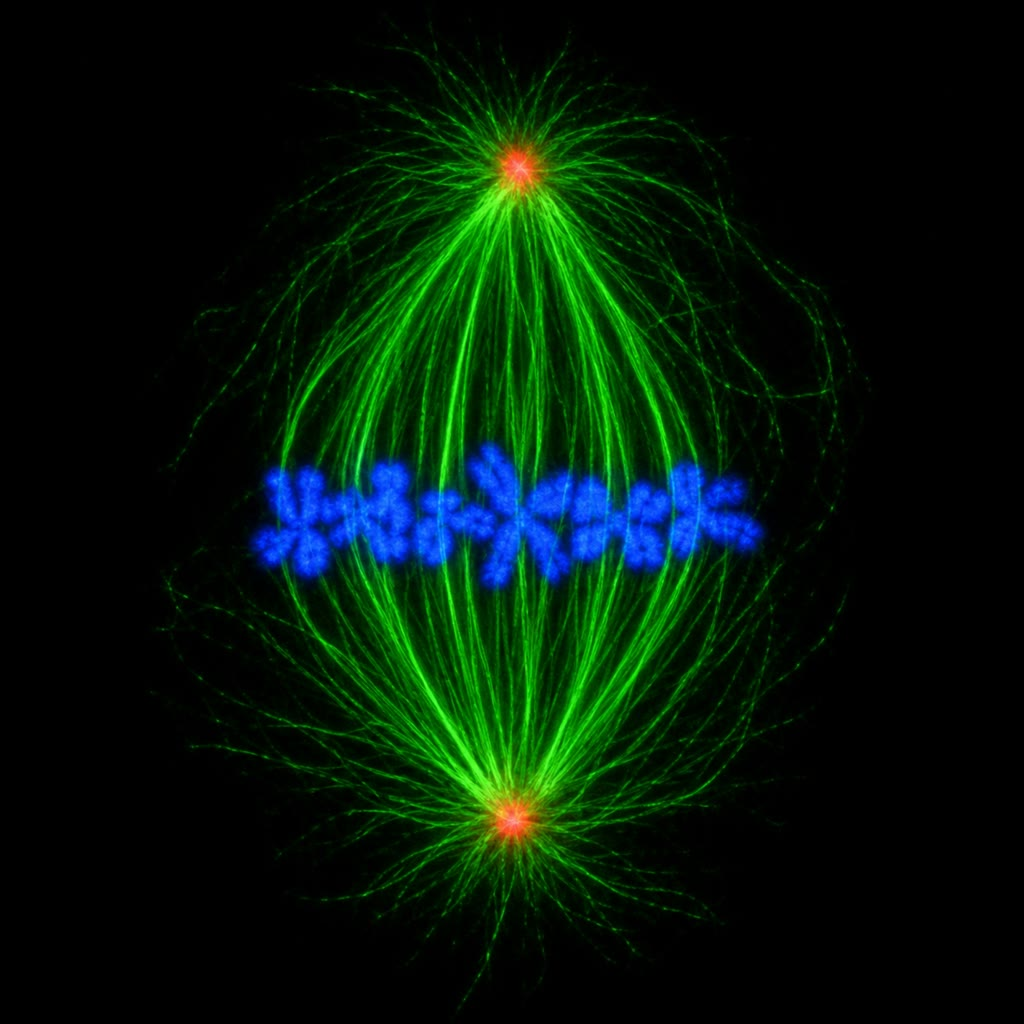
\includegraphics[width=0.36\linewidth]{images/book5/ai/b5-10-mitotic-spindle.jpg}\hspace{0.04\linewidth}
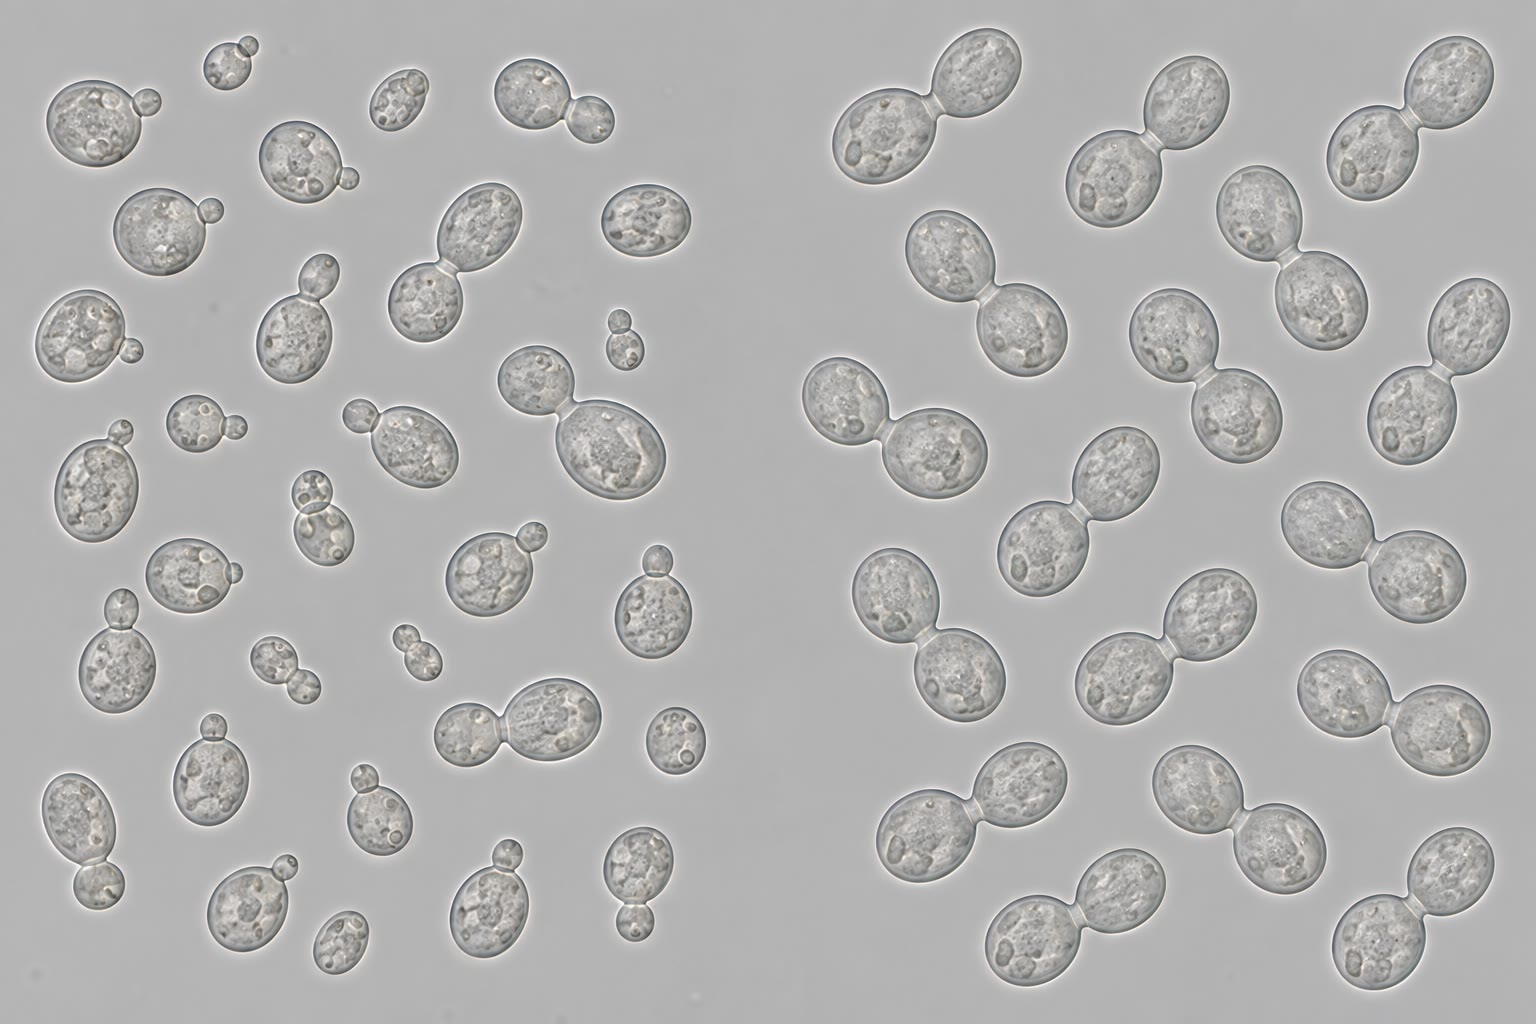
\includegraphics[width=0.54\linewidth]{images/book5/ai/b5-10-yeast-cdc-mutants.jpg}

{\small Izquierda: una célula en metafase --- los \omterm{def:b3:cytoskeleton-motility:filaments}{microtúbulos} del huso
(verde) desde los dos polos (rojo), los cromosomas (azul) alineados en la
placa, el momento en que decide el \omterm{def:b3:cell-cycle-apoptosis:checkpoints}{punto de control} del huso. Derecha:
levadura de gemación, silvestre con yemas de todos los tamaños
(izquierda) y un mutante \emph{cdc} en el que todas las células se han
detenido en la misma etapa, cada una con una yema del mismo tamaño
(derecha).}
\end{omfigure}

\section{La apoptosis}

\begin{definition}[Apoptosis]\label{def:b3:cell-cycle-apoptosis:apoptosis}
\index{apoptosis}\index{necrosis}\index{caspasa}\index{fosfatidilserina}
La \emph{apoptosis} es la muerte celular programada por una secuencia
intrínseca: la célula se encoge y se redondea, su \omterm{def:b3:chromatin-epigenetics:nucleosome}{cromatina} se condensa y
su ADN se corta entre \omterm{def:b3:chromatin-epigenetics:nucleosome}{nucleosomas} en una escalera de fragmentos, el
núcleo se rompe, la membrana forma ampollas selladas, la fosfatidilserina
aparece en la cara externa de la membrana como señal de ``cómeme'', y los
fragmentos los engullen las vecinas o los macrófagos en menos de una hora
--- sin fugas y, por tanto, sin inflamación. La ejecutan las
\emph{caspasas}, cisteína-proteasas que cortan detrás de un aspartato y
se fabrican como zimógenos inactivos: las caspasas \emph{iniciadoras}
(8 y 9) se activan al juntarse sobre una plataforma, y cortan y activan a
las caspasas \emph{ejecutoras} (3 y 7), que cortan varios centenares de
sustratos --- las laminas, el citoesqueleto, el inhibidor de la nucleasa
que corta el ADN, la enzima que mantiene dentro la fosfatidilserina. La
\emph{necrosis}, en cambio, es la muerte por lesión: la célula se hincha,
estalla, derrama su contenido y provoca inflamación. La apoptosis la
bautizaron y describieron morfológicamente Kerr, Wyllie y Currie (1972);
sus genes se encontraron en un gusano.
\end{definition}

\begin{proof}[Evidencia]
Todo hermafrodita de \emph{Caenorhabditis elegans} fabrica $1090$ células
somáticas, de las que mueren siempre las mismas $131$, cada una en un
momento y un lugar fijos. Horvitz y colaboradores (años ochenta) aislaron
mutantes en los que sobrevivían: \emph{ced-3} y \emph{ced-4} hacían falta
para todas las muertes, y en su ausencia las $131$ células vivían y se
diferenciaban; \emph{ced-9} protegía --- su pérdida mataba células que
debían vivir, y su exceso de actividad salvaba células que debían morir
---; y \emph{egl-1} hacía falta para muertes concretas. CED-3 era una
\omterm{def:b3:cell-cycle-apoptosis:apoptosis}{caspasa}, CED-4 su plataforma de activación (Apaf-1 en el ser humano),
CED-9 una proteína Bcl-2 y EGL-1 una proteína solo-BH3: la vía humana,
gen por gen. El propio gen humano \emph{BCL2} se había encontrado en una
translocación cromosómica del linfoma folicular, un cáncer de células que
no consiguen morir.
\end{proof}

\begin{definition}[Las dos vías]\label{def:b3:cell-cycle-apoptosis:pathways}
\index{vía intrínseca}\index{vía extrínseca}\index{familia Bcl-2}\index{citocromo c}\index{apoptosoma}\index{receptor de muerte}
La vía \emph{intrínseca} (mitocondrial) integra el estado interno de la
célula. La \emph{familia Bcl-2} tiene tres clases: los guardianes
(Bcl-2, Bcl-xL, Mcl-1), que se sitúan en la membrana externa mitocondrial
y la mantienen sellada; los efectores (Bax, Bak), que, al activarse,
oligomerizan en poros de esa membrana; y los sensores \emph{solo-BH3}
(Bim, Bid, Puma, Noxa, Bad), cada uno inducido o activado por un daño
concreto --- el daño del ADN a través de p53 (Puma, Noxa), la retirada
del factor de crecimiento (Bim, Bad), el desprendimiento, las proteínas
mal plegadas ---, que se unen a los guardianes y liberan o activan a los
efectores. Cuando ganan los efectores, la membrana externa se
permeabiliza, el \emph{citocromo~c} se escapa al citosol, se une a Apaf-1
y forma el \emph{apoptosoma}, que activa a la \omterm{def:b3:cell-cycle-apoptosis:apoptosis}{caspasa}~9. La vía
\emph{extrínseca} empieza fuera: los \emph{receptores de muerte} (Fas, el
receptor de TNF, los receptores de TRAIL), unidos por sus ligandos de un
linfocito asesino o de una vecina, se agrupan, reclutan adaptadores y
activan a la \omterm{def:b3:cell-cycle-apoptosis:apoptosis}{caspasa}~8, que corta directamente a la \omterm{def:b3:cell-cycle-apoptosis:apoptosis}{caspasa}~3 y, a través
de Bid, abre también la ruta mitocondrial. Las dos vías convergen en las
\omterm{def:b3:cell-cycle-apoptosis:apoptosis}{caspasas} ejecutoras, y unas proteínas inhibidoras (IAP, FLIP) fijan el
umbral por el camino.
\end{definition}

\begin{omfigure}
\begin{tikzpicture}[every node/.style={font=\scriptsize}, >=stealth]
  % extrinsic
  \node[draw, thick, rounded corners, fill=omProp!25, align=center] (lig) at (0,4.2) {ligando de muerte en una célula asesina\\(FasL, TNF, TRAIL)};
  \node[draw, thick, rounded corners, fill=omProp!25, align=center] (rec) at (0,2.8) {los receptores de muerte se agrupan;\\los adaptadores reclutan la caspasa-8};
  \node[draw, thick, rounded corners, fill=omThm!20] (c8) at (0,1.5) {caspasa-8 activa};
  % intrinsic
  \node[draw, thick, rounded corners, fill=omDef!20, align=center] (insult) at (7.2,4.2) {daño en el ADN (p53), pérdida de factor de crecimiento,\\desprendimiento, proteínas mal plegadas};
  \node[draw, thick, rounded corners, fill=omDef!20, align=center] (bh3) at (7.2,3.0) {los sensores solo-BH3 (Puma, Bim, Bid)\\neutralizan Bcl-2 y activan Bax/Bak};
  \node[draw, thick, rounded corners, fill=omDef!20, align=center] (mito) at (7.2,1.7) {la membrana externa mitocondrial se abre:\\sale el citocromo $c$, se forma el apoptosoma};
  \node[draw, thick, rounded corners, fill=omThm!20] (c9) at (7.2,0.5) {caspasa-9 activa};
  % convergence
  \node[draw, thick, rounded corners, fill=omThm!35, align=center] (c3) at (3.6,-0.8) {caspasas ejecutoras 3 y 7:\\cortan centenares de sustratos};
  \node[draw, thick, rounded corners, fill=gray!15, align=center] (out) at (3.6,-2.3) {cromatina condensada, ADN en escalera, ampollas,\\fosfatidilserina expuesta, engullida};
  \draw[->, thick] (lig) -- (rec); \draw[->, thick] (rec) -- (c8); \draw[->, thick] (c8) -- (c3);
  \draw[->, thick] (insult) -- (bh3); \draw[->, thick] (bh3) -- (mito); \draw[->, thick] (mito) -- (c9); \draw[->, thick] (c9) -- (c3);
  \draw[->, thick] (c3) -- (out);
  \draw[->, thick, dashed] (c8) -- (bh3) node[pos=0.55, below, sloped] {Bid cortada: las dos rutas se unen};
  \node[left, omThm, align=right] at (-2.3,1.5) {vía\\extrínseca}; \node[right, omDef, align=left] at (10.4,1.7) {vía\\intrínseca};
  \node[right, font=\tiny, align=left] at (8.6,0.5) {las IAP inhiben aquí;\\Bcl-2 vigila más arriba};
\end{tikzpicture}

{\small Las dos rutas hacia las \omterm{def:b3:cell-cycle-apoptosis:apoptosis}{caspasas} ejecutoras. De fuera adentro, un
\omterm{def:b3:cell-cycle-apoptosis:pathways}{receptor de muerte} activa la caspasa-8; de dentro afuera, la \omterm{def:b3:cell-cycle-apoptosis:pathways}{familia
Bcl-2} sopesa el estado de la célula y, cuando ganan los efectores, la
mitocondria libera el citocromo~$c$ y se activa la caspasa-9. Ambas
convergen en la caspasa-3.}
\end{omfigure}

\begin{proposition}[El punto de no retorno]\label{prop:b3:cell-cycle-apoptosis:mompt}
\index{permeabilización de la membrana externa mitocondrial}
La \omterm{prop:b3:cell-cycle-apoptosis:mompt}{permeabilización de la membrana externa mitocondrial} es repentina ---
todas las mitocondrias de una célula se abren en unos cinco minutos, tras
horas de deliberación --- y completa: una vez que el citocromo~$c$ está
en el citosol, la activación de las \omterm{def:b3:cell-cycle-apoptosis:apoptosis}{caspasas} llega en minutos y no puede
deshacerse retirando el estímulo. Dos rasgos la convierten en un
interruptor. El poro de Bax/Bak se forma por oligomerización, de modo que
su velocidad sube abruptamente con la cantidad de efector activado; y los
guardianes y los sensores se unen entre sí con alta afinidad, de manera
que hasta un umbral todo sensor queda neutralizado y más allá de él todo
sensor adicional queda libre --- una valoración, como un tampón que se
agota. La célula no muere por tanto de forma gradual; acumula proteínas
solo-BH3 hasta cruzar un umbral, y entonces muere de golpe. Los fármacos
que imitan a las proteínas BH3 (el venetoclax, que ocupa a Bcl-2)
empujan más allá del umbral a las células ``cebadas'' --- ya cerca de él,
como lo están muchas células leucémicas --- y respetan a las que no lo
están.
\end{proposition}

\begin{omfigure}
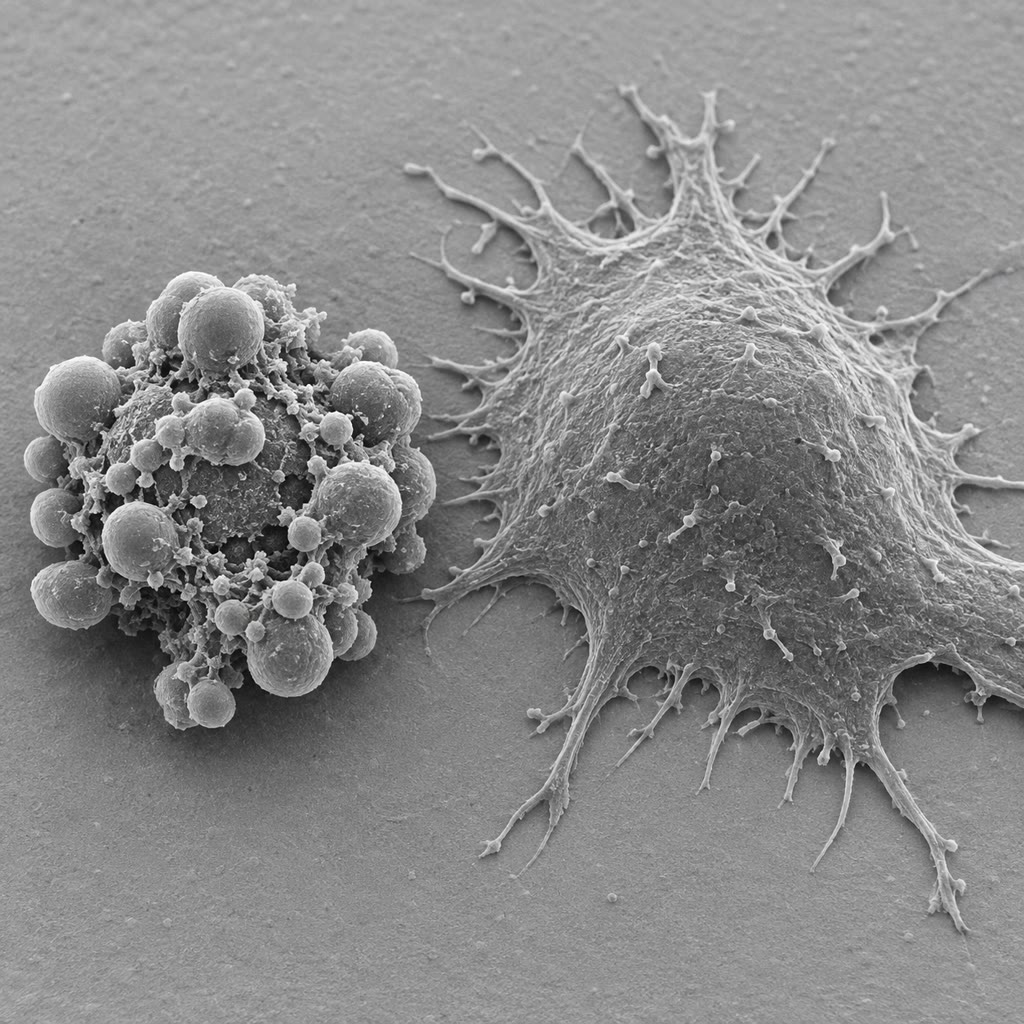
\includegraphics[width=0.40\linewidth]{images/book5/ai/b5-10-apoptotic-cell.jpg}

{\small Una célula apoptótica junto a otra sana en el microscopio
electrónico de barrido: encogida, con la superficie rota en ampollas
selladas que serán engullidas sin rastro de inflamación.}
\end{omfigure}

\begin{example}[Muertes que construyen un cuerpo]\label{ex:b3:cell-cycle-apoptosis:development}
Los dedos se tallan a partir de una paleta mediante la \omterm{def:b3:cell-cycle-apoptosis:apoptosis}{apoptosis} de las
células que hay entre ellos; en el pato esas mismas células viven y la
membrana interdigital permanece. La cola del renacuajo se reabsorbe en la
metamorfosis a la señal de la hormona tiroidea. Alrededor de la mitad de
las neuronas producidas en el sistema nervioso de un vertebrado mueren
antes del nacimiento, las que no reciben suficiente factor trófico de sus
dianas --- una competencia que ajusta el número de neuronas al tamaño del
campo al que sirven. El noventa y cinco por ciento de los linfocitos~T
fabricados en el timo mueren allí, descartados por la selección porque no
reconocen nada o porque reconocen lo propio
(\cref{ch:b3:adaptive-immunity}). Y cada día el epitelio intestinal
desprende sus células más viejas en las puntas de las vellosidades, la
piel sus queratinocitos y la sangre sus neutrófilos envejecidos tras una
vida de un día: la \omterm{def:b3:cell-cycle-apoptosis:apoptosis}{apoptosis} es la rutina, y el tamaño de un tejido es la
diferencia entre dos velocidades grandes.
\end{example}

\section{Otras salidas, y el no saber salir}

\begin{definition}[Necrosis regulada y senescencia]\label{def:b3:cell-cycle-apoptosis:other}
\index{necroptosis}\index{piroptosis}\index{senescencia}
Las células tienen otras muertes programadas, todas inflamatorias allí
donde la \omterm{def:b3:cell-cycle-apoptosis:apoptosis}{apoptosis} es silenciosa. La \emph{necroptosis}, desencadenada
por los \omterm{def:b3:cell-cycle-apoptosis:pathways}{receptores de muerte} cuando la caspasa-8 está bloqueada (como la
bloquean algunos virus), ensambla la quinasa RIPK3 con MLKL, que perfora
la membrana plasmática. La \emph{piroptosis}, en macrófagos infectados,
la ejecuta la caspasa-1 del inflamasoma (\cref{ch:b3:innate-immunity}),
que corta la gasdermina y la convierte en formadora de poros y libera
interleucina-1. La \emph{ferroptosis} es la muerte por peroxidación
lipídica dependiente de hierro. Una célula puede además dejar de
dividirse sin morir: la \emph{senescencia} es una parada permanente,
impuesta por p16 y p21 tras la erosión de los telómeros
(\cref{ch:b3:stem-cells}), un daño persistente del ADN o la activación de
un oncogén, en la que la célula sigue metabólicamente activa y secreta
factores inflamatorios. La senescencia retira células dañadas de la
reserva que se divide --- un supresor de tumores --- y se acumula con la
edad, donde sus secreciones contribuyen a la degeneración de los tejidos;
eliminar las células senescentes en ratones alarga la vida sana.
\end{definition}

\begin{remark}[Demasiado poco y demasiado]\label{rem:b3:cell-cycle-apoptosis:disease}
Las enfermedades de estos programas son de dosis. Demasiada poca muerte:
el cáncer, en el que el umbral apoptótico sube por la sobreexpresión de
Bcl-2 o la pérdida de p53, de modo que células con el genoma dañado
sobreviven para acumular más daño; y la autoinmunidad, cuando persisten
linfocitos que debieron morir en la selección. Demasiada: la pérdida de
linfocitos~T en la infección por el VIH, las neuronas de la penumbra de
un ictus que mueren por \omterm{def:b3:cell-cycle-apoptosis:apoptosis}{apoptosis} horas después de la isquemia (una
ventana para el tratamiento), la \omterm{def:b3:cell-cycle-apoptosis:apoptosis}{apoptosis} lenta de las neuronas en las
enfermedades neurodegenerativas, las células cardíacas perdidas tras un
infarto. El tratamiento del cáncer es en gran medida la inducción
deliberada de \omterm{def:b3:cell-cycle-apoptosis:apoptosis}{apoptosis} en células cuyos umbrales son más bajos que los
de sus vecinas, y los fármacos que atacan a Bcl-2 y a Cdk4/6 son los
primeros diseñados a partir de los mapas de este capítulo.
\end{remark}

\section{Ejercicios}

\begin{exercise}[$\star$]\label{exo:b3:cell-cycle-apoptosis:1}
Enumérense las cuatro fases del ciclo, la pareja ciclina--CDK que impulsa
cada transición y la ubiquitina-ligasa que termina la mitosis.
\end{exercise}

\begin{exercise}[$\star$]\label{exo:b3:cell-cycle-apoptosis:2}
¿Qué aportó cada uno de Hartwell, Nurse y Hunt al descubrimiento del
motor, y en qué organismo?
\end{exercise}

\begin{exercise}[$\star$]\label{exo:b3:cell-cycle-apoptosis:3}
Nómbrense los tres \omterm{def:b3:cell-cycle-apoptosis:checkpoints}{puntos de control}, la condición que comprueba cada uno
y la diana molecular sobre la que actúa cada uno.
\end{exercise}

\begin{exercise}[$\star$]\label{exo:b3:cell-cycle-apoptosis:4}
Distíngase la \omterm{def:b3:cell-cycle-apoptosis:apoptosis}{apoptosis} de la \omterm{def:b3:cell-cycle-apoptosis:apoptosis}{necrosis} en cinco rasgos, y nómbrese la
clase de enzima que ejecuta la \omterm{def:b3:cell-cycle-apoptosis:apoptosis}{apoptosis}.
\end{exercise}

\begin{exercise}[$\star\star$]\label{exo:b3:cell-cycle-apoptosis:5}
En un extracto de huevo de rana la \omterm{def:b3:cell-cycle-apoptosis:cdk}{ciclina} B se sintetiza a
$k_{s} = 1$ unidad por minuto; el umbral mitótico es $C_{2} = 30$
unidades, el umbral de salida $C_{1} = 5$, y en mitosis la \omterm{def:b3:cell-cycle-apoptosis:cdk}{ciclina} se
degrada con una semivida de \qty{2}{min}. Estímense el período de la
oscilación y la fracción del ciclo pasada en mitosis.
\end{exercise}

\begin{exercise}[$\star\star$]\label{exo:b3:cell-cycle-apoptosis:6}
Predígase el comportamiento de una célula (a) que expresa una \omterm{def:b3:cell-cycle-apoptosis:cdk}{ciclina} B
no degradable, (b) que carece de Wee1, (c) que carece de Cdc25, (d) que
expresa una Cdk1 que Wee1 no puede fosforilar, en términos del oscilador
del \cref{thm:b3:cell-cycle-apoptosis:oscillator}.
\end{exercise}

\begin{exercise}[$\star\star$]\label{exo:b3:cell-cycle-apoptosis:7}
Una fusión de Rao y Johnson une una célula en G1 con una en fase S; otra
une una célula en G2 con una en fase S. Predígase lo que hace cada núcleo
y explíquese con la licencia y los niveles de CDK.
\end{exercise}

\begin{exercise}[$\star\star$]\label{exo:b3:cell-cycle-apoptosis:8}
Explíquese por qué un solo cinetocoro sin unir puede retener la anafase
de toda la célula, y predígase el destino de una célula en la que se ha
suprimido Mad2.
\end{exercise}

\begin{exercise}[$\star\star$]\label{exo:b3:cell-cycle-apoptosis:9}
Predígase el fenotipo de un gusano sin \emph{ced-9}; sin \emph{ced-3};
sin ambos. Explíquese la epistasis en términos de la vía.
\end{exercise}

\begin{exercise}[$\star\star\star$]\label{exo:b3:cell-cycle-apoptosis:10}
Muéstrese que un solo bucle de retroalimentación negativa sin
interruptor biestable --- \omterm{def:b3:cell-cycle-apoptosis:cdk}{ciclina} sintetizada a $k_{s}$, degradada a
$k_{d}AC$ con $A$ simplemente proporcional a $C$ --- tiene un estado
estacionario estable y no oscila. ¿Qué añade la curva en forma de S, y
qué añadiría en su lugar un retraso?
\end{exercise}

\begin{exercise}[$\star\star\star$]\label{exo:b3:cell-cycle-apoptosis:11}
Una célula tiene $N$ moléculas del guardián Bcl-2 y recibe sensores
solo-BH3 a una velocidad $r$ por hora tras un estímulo lesivo, y cada
sensor une un guardián. Explíquese por qué la célula muere hacia el
instante $N/r$ sea cual sea la intensidad del estímulo por encima de eso,
por qué la muerte es repentina y qué le hace al tiempo el venetoclax.
\end{exercise}

\begin{exercise}[$\star\star\star$]\label{exo:b3:cell-cycle-apoptosis:12}
El linfoma folicular lleva una translocación que sobreexpresa
\emph{BCL2}; sus células se dividen despacio. El retinoblastoma lleva la
pérdida de \emph{RB}; sus células se dividen deprisa. Explíquese cómo
cada lesión aislada produce un tumor, por qué el primero es indolente y
el segundo agresivo, y qué dice cada uno sobre los dos programas de este
capítulo.
\end{exercise}

\section{Problema: la vida y la muerte de un epitelio}

\begin{problem}[{Problema de fin de semana --- el revestimiento
intestinal renovado célula a célula, el ciclo cronometrado con el
oscilador de la ciclina, los errores de un punto de control contados en
todo un cuerpo y la eliminación por apoptosis de cien mil millones de
células al día pesada, hasta llegar al período del ciclo, a las células
aneuploides producidas al día y a la masa que el cuerpo recicla por
apoptosis}]
\label{pb:b3:cell-cycle-apoptosis:1}
Datos: el intestino delgado tiene $10^{7}$ criptas, y cada una renueva
una vellosidad de \num{3500} células cada $5$ días; cada cripta alberga
unas $22$ células madre que se dividen una vez al día y cuya progenie se
divide $5$ veces más antes de diferenciarse. Oscilador: $k_{s} = 2$
unidades de \omterm{def:b3:cell-cycle-apoptosis:cdk}{ciclina} por hora, $C_{2} = 40$ unidades, $C_{1} = 8$,
semivida mitótica de la \omterm{def:b3:cell-cycle-apoptosis:cdk}{ciclina} \qty{10}{min}. \omterm{def:b3:cell-cycle-apoptosis:checkpoints}{Punto de control}: sin el
\omterm{def:b3:cell-cycle-apoptosis:checkpoints}{punto de control} del huso, una división de cada $50$ segrega mal un
cromosoma; con él, una de cada \num{50000}. El cuerpo repone $10^{11}$
células al día de \qty{1}{ng} de masa cada una, con un \qty{20}{\%} de
proteína; un macrófago elimina una célula apoptótica en \qty{1}{h}.

\medskip
\noindent\textbf{Parte I --- Renovación.}
\begin{enumerate}
  \item ¿Cuántas células desprende el intestino delgado al día, y por
        segundo?
  \item ¿Cuántas células produce una cripta al día? Compruébese: $22$
        divisiones de células madre al día, y cada hija comprometida
        dividiéndose $5$ veces más.
  \item Si una célula madre se divide una vez al día durante una vida de
        $80$ años, ¿cuántas divisiones? Con una tasa de mutación de $0.6$
        por genoma y división (\cref{ch:b3:dna-repair}), ¿cuántas
        mutaciones acumula?
  \item Las células de tránsito se dividen cada \qty{12}{h}. ¿Por qué
        puede el tejido permitirse divisiones de tránsito rápidas y de
        vida corta, pero mantiene lenta a la célula madre?
  \item Una dosis de radiación mata todas las células de tránsito que se
        dividen pero respeta a las células madre, que se reanudan en un
        día. ¿Cuánto tarda la vellosidad, sin reposición, en quedar
        desnuda, y cuánto se tarda en reconstruirla? ¿Por qué es el
        intestino una víctima temprana de la radiación?
  \item En el colon el desprendimiento de la parte alta es por \omterm{def:b3:cell-cycle-apoptosis:apoptosis}{apoptosis}
        (anoikis, la muerte al desprenderse). ¿Por qué es este el modo de
        muerte adecuado para una célula en contacto con las bacterias del
        intestino?
\end{enumerate}

\medskip
\noindent\textbf{Parte II --- El reloj.}
\begin{enumerate}[resume]
  \item Con los datos del oscilador, ¿cuánto tarda la \omterm{def:b3:cell-cycle-apoptosis:cdk}{ciclina} en subir de
        $C_{1}$ a $C_{2}$?
  \item ¿Cuánto tarda la degradación mitótica en bajarla de $C_{2}$ de
        vuelta a $C_{1}$?
  \item Período del oscilador desnudo, y fracción del período con Cdk1
        activa.
  \item Las células de tránsito de la cripta ciclan en \qty{12}{h}, las
        células madre en \qty{24}{h} y el huevo de rana en \qty{30}{min}.
        ¿Cuál de los parámetros del modelo difiere, y qué aporta la
        diferencia en una célula somática?
  \item Una célula detenida en el \omterm{def:b3:cell-cycle-apoptosis:checkpoints}{punto de control} G2/M por un daño en el
        ADN sigue fabricando \omterm{def:b3:cell-cycle-apoptosis:cdk}{ciclina} B. ¿Dónde está en el plano de fases,
        y qué la mantiene ahí? ¿Qué ocurre cuando se repara el daño?
  \item Un fármaco inhibe el APC/C. Descríbase el destino de una célula
        que entra en mitosis en su presencia.
\end{enumerate}

\medskip
\noindent\textbf{Parte III --- Errores.}
\begin{enumerate}[resume]
  \item ¿Cuántas divisiones al día lleva a cabo el cuerpo para reponer
        $10^{11}$ células?
  \item ¿Cuántas hijas aneuploides al día con el \omterm{def:b3:cell-cycle-apoptosis:checkpoints}{punto de control}, y
        cuántas sin él?
  \item La mayoría de las células aneuploides mueren o se detienen (p53
        responde a la mala segregación). Si sobrevive el \qty{1}{\%} y se
        divide, ¿cuántas células aneuploides en división produce al día
        un cuerpo con el \omterm{def:b3:cell-cycle-apoptosis:checkpoints}{punto de control} intacto, y cuántas a lo largo
        de una vida?
  \item Un tumor de $10^{9}$ células ha perdido el \omterm{def:b3:cell-cycle-apoptosis:checkpoints}{punto de control} y
        p53. ¿Cuántas malas segregaciones al día lleva a cabo, y por qué
        esto lo hace evolucionar deprisa?
  \item Explíquese por qué la pérdida completa del \omterm{def:b3:cell-cycle-apoptosis:checkpoints}{punto de control} del
        huso es letal para un embrión aunque la pérdida parcial favorezca
        el cáncer.
  \item El síndrome de Down surge de una mala segregación en la meiosis,
        no en la mitosis. Explíquese por qué un error en una sola célula
        allí afecta a todas las células del niño, mientras que un error
        mitótico afecta a un solo linaje.
\end{enumerate}

\medskip
\noindent\textbf{Parte IV --- Eliminación.}
\begin{enumerate}[resume]
  \item ¿Qué masa de células elimina el cuerpo por \omterm{def:b3:cell-cycle-apoptosis:apoptosis}{apoptosis} al día, y al
        año? Compárese con la masa corporal.
  \item ¿Cuánta proteína es eso al día? Compárese con una ingesta
        alimentaria de \qty{70}{g}: ¿qué fracción del recambio proteico
        del cuerpo es el reciclado de células muertas?
  \item ¿Cuántos macrófagos, trabajando sin descanso, hacen falta para
        eliminar los muertos de un día? El cuerpo tiene unos $10^{11}$
        macrófagos: ¿qué fracción de su tiempo?
  \item ¿Por qué hay que retirar el cadáver antes de que se lise, y qué
        señales dicen ``cómeme''?
  \item Un paciente sobreexpresa Bcl-2 en sus linfocitos~B. ¿Qué vía
        queda bloqueada? ¿Funciona todavía la \omterm{def:b3:cell-cycle-apoptosis:pathways}{vía extrínseca}? ¿Por qué el
        resultado es un linfoma de crecimiento lento y no uno rápido?
  \item Las neuronas de la penumbra de un ictus mueren por \omterm{def:b3:cell-cycle-apoptosis:apoptosis}{apoptosis}
        entre seis y veinticuatro horas después del insulto, y las del
        núcleo por \omterm{def:b3:cell-cycle-apoptosis:apoptosis}{necrosis} en cuestión de minutos. ¿Por qué la primera
        ofrece una ventana para el tratamiento y la segunda ninguna?
  \item Resúmase: el período del oscilador desnudo (pregunta~9), las
        células aneuploides en división al día en un cuerpo normal
        (pregunta~15) y la masa reciclada por \omterm{def:b3:cell-cycle-apoptosis:apoptosis}{apoptosis} al día
        (pregunta~19).
\end{enumerate}
\end{problem}
